\RequirePackage[l2tabu, orthodox]{nag}
\documentclass[12pt,a4paper,naustrian,english,oneside,openright,DIV=12,BCOR=1cm]{scrbook}

\usepackage[T1]{fontenc}
\usepackage[utf8]{inputenc}

\usepackage{fancyhdr}
\pagestyle{fancy}
\setcounter{secnumdepth}{3}
\usepackage{babel}
\usepackage{textcomp}
\usepackage{url}
\usepackage{makeidx}
\makeindex
\usepackage{graphicx}
\PassOptionsToPackage{normalem}{ulem}
\usepackage{ulem}
\usepackage{booktabs}
\usepackage{minted}
\usepackage{xcolor}
\newcommand\crule[3][black]{\color{#1}{\rule{#2}{#3}}}
\usepackage{soul}
\usepackage{amssymb}
\usepackage{float}
\usepackage{placeins}

\setminted{autogobble,linenos,tabsize=4}

\usepackage[
	unicode=true,
	bookmarks=true,
	bookmarksnumbered=false,
	bookmarksopen=false,
	breaklinks=true,
	pdfborder={0 0 0},
	backref=false,
	colorlinks=false
]{hyperref}
\hypersetup{%
	pdftitle={File Tagger},
	pdfauthor={%
		Christoph Führer,
		Julian Lorenz,
		Erik Ritschl,
		Clemens Stadlbauer
	},
	pdfsubject={Diplomarbeit},
	pdfkeywords={dies, das} % TODO
}
\usepackage{cleveref}

% Latex-Vorspann
\usepackage{lastpage}
\usepackage{blindtext}

% Tweaks
%\usepackage{geometry} TODO
\usepackage{microtype}
\usepackage{enumitem}
\setitemize{leftmargin=*}

% Font
%\usepackage{caladea}
%\usepackage{lmodern}
\usepackage{mathpazo}
\usepackage[resetfonts]{cmap} % make pdf searchable

\frenchspacing
\graphicspath{%
	{./images/}
}

\begin{document}
%%%%%%
% Weitere Einstellungen siehe Latex-Vorspann
% falls man die erste Zeile der Absätze nicht einrücken will
% dann sollte man aber etwas mehr Abstand zwischen den Absätzen erlauben
%%\setlength{\parindent}{0pt}
%%\setlength{\parskip}{1.5ex plus0.5ex minus0.5ex}
% Auch Fußnoten bündig ausrichten
\deffootnote[]{1em}{1em}{\textsuperscript{\thefootnotemark\ }}

% Header and Footer
\newcommand{\kopfseitenummer}{{\bfseries \thepage}}
\newcommand{\kopfkapl}{{\bfseries\leftmark}}
\newcommand{\kopfkapr}{{\bfseries\rightmark}}
\newcommand{\kopfbild}{
\includegraphics[width=25mm]{htl3r-logo}}
\newcommand{\kopfHTL}{%
	Höhere Technische Bundeslehranstalt Wien 3, \\
	Rennweg Abteilung für Informationstechnologie
}
\renewcommand{\chaptermark}[1]%
  {\thispagestyle{fancy}\markboth{\thechapter.\ #1}{}}
\renewcommand{\headrulewidth}{0pt}
%\lhead[\fancyplain{\kopfbild}{\kopfbild}]% li aussen
%      {\fancyplain{\kopfHTL}{\kopfHTL}}% re innen
%\rhead[\kopfHTL]% li innen
%      {\kopfbild}% re aussen

\def\kapitelautor{}
% TODO move kapitelautor next to header

% \<left or right side><head or foot>[even side]{odd side}
\lhead[\kopfbild]{\kopfkapl}
\rhead[\kopfkapr]{\kopfbild}
\chead{}

\lfoot%
[\kopfseitenummer]%
{\ifx \kapitelautor \empty {} \else Author: \kapitelautor \fi}
\rfoot%
[\ifx \kapitelautor \empty {} \else Author: \kapitelautor \fi]%
{\kopfseitenummer}
\cfoot[]{}

% Anfang Titelseite
\pagenumbering{roman}
\title{Diplomarbeit}
\selectlanguage{naustrian}
\begin{titlepage}
\begin{minipage}[b]{1\columnwidth}
\parbox[b]{50mm}{
\includegraphics[width=45mm]{images/htl3r-logo}}
\hfill
\parbox[b]{130mm}{\footnotesize \textsc{Höhere Technische Bundeslehranstalt} Wien 3, Rennweg\\
IT \& Mechatronik\\
\\
HTL Rennweg :: Rennweg 89b\\
A-1030 Wien :: Tel +43 1 24215-10 :: Fax DW 18
}\\
\mbox{}
\end{minipage}

\vspace{1cm}


% TODO
\begin{center}
\textbf{\LARGE{}Diplomarbeit}{\large{}}\\
{\large{}\vspace{15mm}
 }
\textbf{\large{}File Tagger}\\
 \vspace{15mm}
 ausgeführt an der\\
 Höheren Abteilung für Informationstechnologie/Ausbildungsschwerpunkt\\
 der Höheren Technischen Lehranstalt Wien 3 Rennweg\\
 \vspace{1cm}
 im Schuljahr 2015/2016\\
 \vspace{1cm}
 durch\\
 \vspace{0.5cm}
\textbf{\large{}Christoph Führer}\\
\textbf{\large{}Julian Lorenz}\\
\textbf{\large{}Erik Ritschl}\\
\textbf{\large{}Clemens Stadlbauer}\\

\par\end{center}{\large \par}

\begin{center}
\vspace{20mm}
 \normalsize unter der Anleitung von\\
 \vspace{0.5cm}
 Ferdinand Kasper\\
Franz Stimpfl\\
Roman Jerabek\\
Martina Oswald \\
\par\end{center}

\begin{center}
\vspace{5mm}
Wien, \today
\par\end{center}

\end{titlepage}%%%%%%%%%%%%%%%%%%%%% Ende Titelseite %%%%%%%%%%%%%%%%%%%%%%
\selectlanguage{english}

\addchap*{Abstract}

% mit Kopfzeile
\thispagestyle{fancy}
In this diploma thesis we describe the planning and execution of our final
school project. It is officially registered as \textit{FileTagger}, but we later changed the name to \textit{OctoTagger}.

OctoTagger is a free and open source desktop application for Windows, Mac OS X and Linux. The
software enables its users to organize their files not by location, but by tags
that describe the contents. The user can assign tags easily via the user
interface, everything else is handled automatically in the background. Every tag has its own folder, and every folder contains links that point to each file with
the according tag.

All file types are supported, be it documents, videos or images. However,
the software is strongly optimized for working with images and photos.

What makes OctoTagger special is that everything is entirely organized via the regular \emph{file system}. So there is no need to open the
application in order to view the files sorted by tags. Users can stick to their regular file browser, and open and edit the files just like they normally would. The software only needs to run in order to assign tags.

% Todo: Folgende Teile in Deutsch oder Englisch?
\addchap*{Ehrenwörtliche Erklärung}

% mit Kopfzeile
\thispagestyle{fancy}

Ich versichere,
\begin{itemize}
\item dass ich meinen Anteil an dieser Diplomarbeit selbstständig verfasst
habe,
\item dass ich keine anderen als die angegebenen Quellen und Hilfsmittel
benutzt habe
\item und mich auch sonst keiner unerlaubten Hilfe bzw. Hilfsmittel bedient
habe.
\end{itemize}
\bigskip{}
Wien, am 31. März 2016 %TODO Aktuelles Datum

\vfill
\noindent\begin{tabular}{p{.45\linewidth}p{.1\linewidth}p{.45\linewidth}}
	\dotfill & & \dotfill \\
	Erik Ritschl & & Clemens Stadlbauer \\[16ex]
	\dotfill & & \dotfill \\
	Christoph Führer & & Julian Lorenz
\end{tabular}
\vfill


\addchap*{Präambel}

\thispagestyle{fancy}

Die Inhalte dieser Diplomarbeit entsprechen den Qualitätsnormen für
``Ingenieurprojekte'' gemäß §\,29 der Verordnung des Bundesministers
für Unterricht und kulturelle Angelegenheiten über die Reife- und
Diplomprüfung in den berufsbildenden höheren Schulen, BGBl. Nr. 847/1992,
in der Fassung der Verordnungen BGBl. Nr. 269/1993, Nr. 467/1996 und
BGBl. II Nr. 123/97.

\vspace{10mm}


Liste der betreuenden Lehrer:

Prof. DI Dr. Ferdinand Kasper, Hauptbetreuer

Prof. DI Franz Stimpfl, Hauptbetreuer Stellvertreter

Prof. Mag. Roman Jerabek, Nebenbetreuer

Prof. Mag. Martina Oswald, Nebenbetreuer % TODO: Englischbetreuer?

\vspace{10mm}

\renewcommand*{\chapterpagestyle}{fancy}
\cleardoublepage{}
\tableofcontents{}
\cleardoublepage{}
\listoftables
\cleardoublepage{}
\listoffigures
\cleardoublepage{}
\listoflistings

\cleardoublepage{}

\pagenumbering{arabic}
\pagestyle{fancy}
\thispagestyle{fancy}

% various semantic \tf (text formatting) commands
\newcommand{\tfpath}[1]{\textbf{#1}}
\newcommand{\tfcode}[1]{\texttt{\detokenize{#1}}}

\chapter{Idea}
\section{Problem}
\def\kapitelautor{Julian Lorenz}

Sometimes it makes sense to categorize files by different criteria so you have to copy the same file to different directories. However, saving files in more than one location at the same time is not recommended because if you change a file, it's hard to synchronise all the different copies.  Additionally, you need more disc space than necessary.

\section{Solution}
\def\kapitelautor{Julian Lorenz}

OctoTagger offers a solution for this problem. The basic feature of this software is to add tags to files and provide access to those files filtered by the attached tags. 

Different folder are created for each tag or combination of different tags and with the help of symbolic links the tagged files can be accessed from those folders without saving them multiple times.

The tags can be managed easily through the OctoTagger User Interface. It is possible to add a single tag with just one click. On the other hand you can also use complex queries containing multiple tags connected with different operators to filter files in OctoTagger. 

OctoTagger is not necessary to run to get access to the tagged files. It is just needed to manage tags and attach them to files.




\chapter{Organization}
\section{Development Methodology}
\def\kapitelautor{Clemens Stadlbauer}

The software development methodology with which this project was developed takes
most of its characteristics from Scrum but also --- even though it seems
contradicting --- some from the Waterfall methodology. Agility and iterative
prototyping is provided by Scrum to ease change management during development.
However, the solid foundation provided by Waterfall provides stability and
helps to focus the development efforts.

% FIXME source
With Waterfall a project is split into these phases: \emph{Pre-Project},
\emph{Rough Planning}, \emph{Fine Planning}, \emph{Development},
\emph{Testing}, \emph{Post-Project}. Each phase strictly requires the previous
phase to be completed.
Due to the school requiring certain documents like an environmental, risk and
requirements analysis, which are usually present in the Waterfall methodology,
it was decided for this project to use the phases as described before but
without the exclusivity. In effect this means that all work during the
beginning of the project roughly fell under \emph{Planning}, all work during
the middle under \emph{Development}, etc. This way a clear, evolving goal is
available for the entire duration of the project.

% FIXME source
In stark contrast to Waterfall, a project utilizing Scrum is split into several
\emph{Sprints} which have a fixed timespan of around 1--2
weeks. At the beginning of the project a \emph{Product Backlog} is created
containing all requirements for the product and at the beginning of each
\emph{Sprint} a general goal is chosen and some tasks from the \emph{Project
Backlog} are moved to the \emph{Sprint Backlog}. At the end of each
\emph{Sprint}, meetings are held to review it and plan the next one.  All
further requirements, like strict meeting guidelines and special management
roles, have been deemed surplus for this project due to the small team size and
the strong time constraint.

\section{Team Roles}
\def\kapitelautor{Clemens Stadlbauer}

Erik Ritschl, who originally had the idea, % TODO cref
also is the project leader. His responsibilities were ensuring Linux
compatibility and implementing new features.

Clemens Stadlbauer is the project leader deputy, whose work was more focused on
the backend.

Christoph Führer is mainly preset in the frontend, where he has implemented
substantial parts of it.

Julian Lorenz, our designer, took on the challenges of creating the Corporate
Design, building the website, writing the user manual and testing the software.

This team was chosen as everyone has a use for the software and the skills
cover every requirement without too much overlap.


\chapter{Result}
\def\kapitelautor{Christoph Führer}
\def\kapitelautor{Christoph Führer}

\section{Structure of the System}
The whole structure of the system should be kept extremely simple. Simplicity was one of the major concerns we had while developing the software because the success of the application relies a lot on being intuitive and simple. Therefore it is just a sole program in a single window which gives the user a very natural feeling when using the application.

All actions performed in the background, for example creating links, database management, assigning tags, \ldots{} are not visible for the user due to the fact that it would further increase the risk of being overwhelmed by OctoTagger's functions.

\section{The final product}
After a lot of hard work we managed to finish the first version of OctoTagger. As mentioned above we made it our business to make it as intuitive as possible. That surely sounds nice but what does it actually mean?

In our case it means that the users have to understand the basic structure of the application quickly. They should be able to easily understand the main mechanics of our software so they can start using it right away. That means any difficulties that the users could experience will hinder their enjoyment and therefore would result in a loss of intuitiveness. The absolute key point on this topic was that the application has to be easy to use for the user, software has to adapt to the users, not the other way around.

To accomplish that we had the idea to make the whole program as native as possible. We wanted to give the users the impression that they are using an application which feels like it is coming directly from the operating system. They should get the experience that there is not even a third party involved. The users should get the feeling that our application is just an extension to their basic file manager, an enhancement which is easy to use and simplifies their file management.

Furthermore, we tried to design every single action that the user may take as simple as possible. Basic commands that the users know from popular programs and operating systems work exactly the same way in OctoTagger. You want to rename a file? Just press \textit{F2}. Refresh the View? Press \textit{F5}. All these classic commands that many of the users are already using by default are implemented precisely the same way in our application so there won't be any conflicts when using OctoTagger. For those not accustomed to shortcuts, there are also buttons for every action and context menus implemented.

When OctoTagger is run for the very first time this is what can be seen:

\begin{figure}[H]
    \centering
    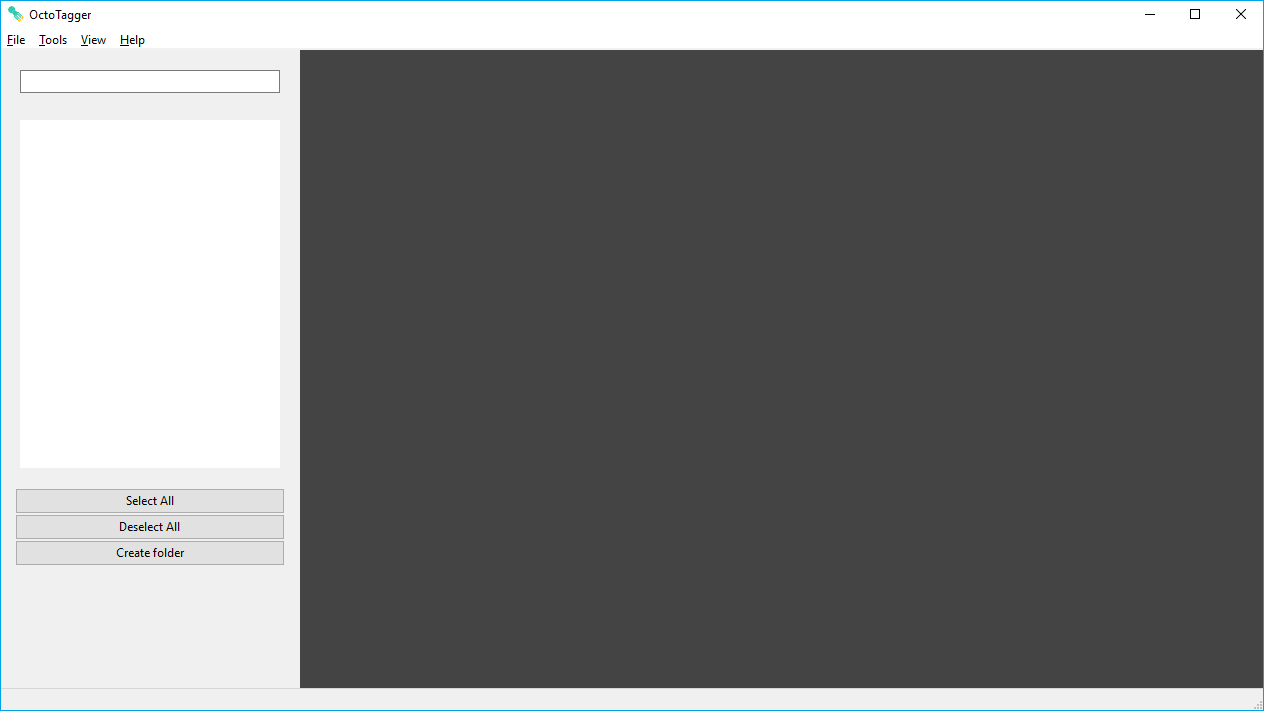
\includegraphics[width=\linewidth]{pp_04}
    \caption{The user interface at startup}
\end{figure}


At this moment it still looks pretty blank. That is because there are neither files imported nor tags assigned yet. To do so, the user has to click on the \emph{File}-Tab and then on one of the file import options.

The next step is to assign tags to the imported files. This is done by selecting the files that are to be tagged, clicking on the tag-bar in the top left corner, typing in a tag and finally pressing Enter. The files are now tagged, which can be seen in the tag-pane right below the tag-bar.
This is an example view of how your application may look like after you are done with the tagging process.

\begin{figure}[H]
    \centering
	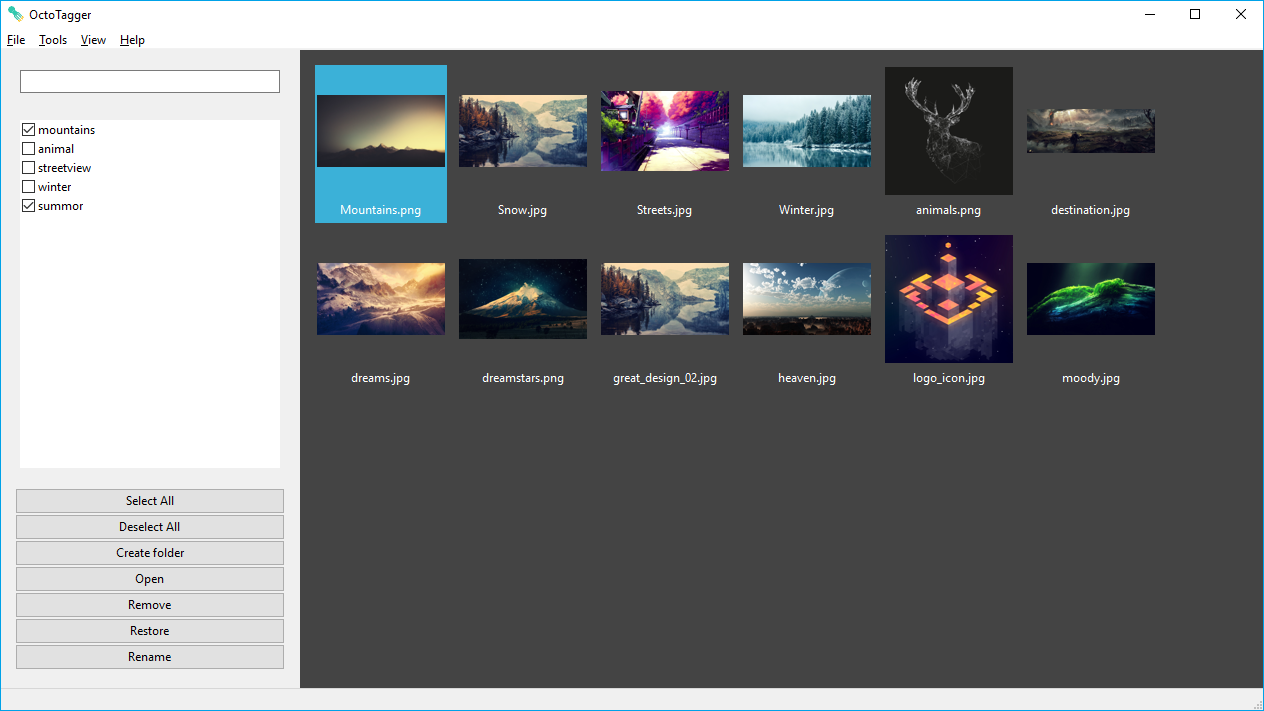
\includegraphics[width=\linewidth]{pp_03}
	\caption{User interface after importing and tagging}
\end{figure}


From this point onwards it is possible to use OctoTagger to its full extent. You can now utilize and enjoy all the different functions that are explained in the forthcoming Implementation chapter (see \cref{ch:mod:implementation}).

\subsection{Behind the scenes}
Now that an impression of the surface has been given, let's take a look at the backend. This is what your folder structure will look like right after downloading and extracting OctoTagger:

\begin{figure}[H]
    \centering
	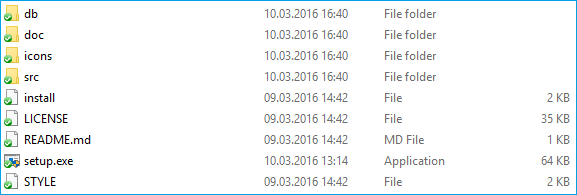
\includegraphics[width=\linewidth]{pp_06}
	\caption{File structure of OctoTagger before installing}
\end{figure}

It really is as simple as it looks. The \emph{db}-folder contains database and SQL files, in the \emph{doc}-folder is our documentation and the user manual, the source files are in the \emph{src}-folder and the \emph{icons}-folder contains logos and other images that are displayed in the application.

\section{Installation}
Installing OctoTagger is easy.

The first step after downloading and extracting the software from our website \url{http://www.octotagger.co/} would be to run the \textit{setup.exe} file on Windows, or the \emph{install} script file on Unix systems. Luckily, this is all that has to be done! Afterwards your directory will look like this:

\begin{figure}[H]
    \centering
	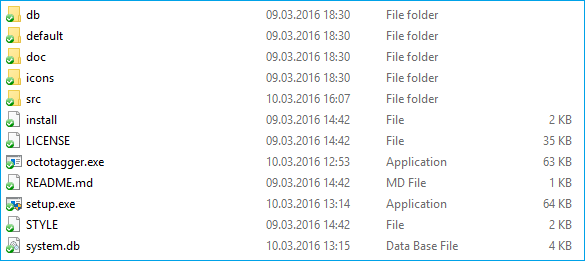
\includegraphics[width=\linewidth]{pp_05}
	\caption{File structure of OctoTagger after installing}
\end{figure}


The following things have changed:
\begin{itemize}
	\item A new folder named \emph{default} has been created. It embodies your default gallery, a \emph{files}-folder, where your imported files are saved, and a \emph{thumbnails}-folder in which the thumbnails for your imported files are saved.
	\item The file \textit{system.db} has been created
	\item An \emph{octotagger.exe} file and a shortcut on the desktop has been created (On Windows)
	\item An \emph{octotagger.desktop} file has been placed in \tfpath{\textasciitilde{}/.local/share/applications} (On Linux) 
	\item You are now able to run OctoTagger!
\end{itemize}

However, it is worth mentioning that you have to execute the setup file with administrator rights under Windows because of the simultaneously created Windows Symlink service which is also explained more in depth in the execution chapter. This is because, under Windows it is necessary to build a service which handles the link creation, due to the fact that Windows does not allow this feature without special permission. By creating a Windows service you only have to grant these rights once and are fine for as long as you keep it installed. If you want to gain a deeper understanding about this topic please consider looking at the \textit{Pywinlink} module section (see \cref{subsec:mod:pywinlink}).

\section{Goals}
We are proud to announce that all mandatory goals have been achieved! The software is running smoothly and we are all utterly satisfied with the outcome of a year of developing OctoTagger. Of course there have been some complications, challenges and other things that did not go exactly as planned, but altogether we did not have any major troubles and had a pleasant time engineering the software.

If you wish to receive more information about the goals achieved, including the optional ones, we recommend the analysis in the \textit{evaluation} chapter (see ). There you will also find information on how we planned the whole project in contrast to how we eventually carried it out.






















\chapter{Implementation}
\section{Theory}
\def \kapitelautor {Christoph Führer}
% TODO explain technical theory

\section{Technologies}
\def \kapitelautor {Christoph Führer}
% TODO explain used technologies

\section{Prototype and Planning} % PoC
\def \kapitelautor {Erik Ritschl}
% TODO chronological order
% function prototypes, learning python
% product backlog
% planning poker
% paper prototype
% code snippets
\subsection{Result} % final prototype

\section{Structure}
\def \kapitelautor {Clemens Stadlbauer}

In our code repository there are several folders, each of which containing a
certain category of files.

\begin{itemize}
	\item[\tfpath{doc/}] The documentation of the software, i.e. the user manual
	\item[\tfpath{icons/}] All the different icons and the logo used throughout the
	software
	\item[\tfpath{db/}] Database schemas and the database setup script
	\item[\tfpath{src/}] The actual code of the software
\end{itemize}

\subsection{db}
In \tfpath{system.sql} is the schema of the main database. It contains the user
settings and the location of all the galleries. Every gallery has its own
database as described in \tfpath{gallery.sql} containing all imported files,
all created tags and all created output folders. The connections between these
items (for example which tags a files has) are recorded in addition,
intermediate tables.

Furthermore, the directory contains a helper script to create the initial
system database and an empty gallery database which is copied every time a new
gallery is created by the user.

\subsection{src}
Herein lie all the modules that make up the entirety of the functionality and
design of OctoTagger. Each module is contained in a single file with the
module's name and can be categorizes as either frontend or backend. All the
frontend modules provide some part of the user interface while all the backend
modules implement mostly all the functionality that happens in the background
(for example the management of files).

% TODO module tree?

\section{Frontend}
%\subsection{Modulename}
\def \kapitelautor {}

\subsubsection{Abstract}

\subsubsection{Attempts}

\subsubsection{Solution} % TODO better title

\section{Backend}
%\subsection{Modulename}
\def \kapitelautor {}

\subsubsection{Abstract}

\subsubsection{Attempts}

\subsubsection{Solution} % TODO better title

% TODO explain code
% each module has a small abstract explaining what and how it works
% each module explained roughly in chronological order

\section{Corporate Design}
%\subsection{Corporate Identity}

What is the first thing you should think about, when you see our logo? Why did we use these colors? Why did we decide to take this font? 

These are just a few questions related to the corporate identity. It determinates how the project team presents itself to the public. Within the corporate identity document everything regarding public appearance can be defined. This could contain the behaviour to the public, as well as communication, philosophy, design, language and much more. 

In case of OctoTagger it was decided to just take care of the design part from the corporate identity, the corporate design. This document contains our design-guidelines for the website. This includes the colors used for the logo and other images, the background colors, the font and the logo itself. 

The challenge at developing a corporate design is to always keep the user in mind. How does the user think? What does he want to see? It's important to attract a potential user and catch his attention. The website is the first thing every potential user gets confronted with, so it has to send the right signals. Colors are great triggers for emotions and feelings making them a powerful tool for the writer of the corporate design. However, the proper combination of the colors is at least as important as the colors themselves. 

The logo design should not be neglected. It's an essential part of the corporate design. The challenge is to design a logo that provides a distinctive look but keeping it as simple as possible at the same time. 

\subsection{Background of the name OctoTagger}

In the beginning there was just the idea for the product, an file organisation software. Afterwards the name OctoTagger was born. The intention behind that name was indeed an octopus and it's ability to handle several actions at the same time, due to his eight arms. In this point OctoTagger and octopuses share similarities. OctoTagger is also able to handle multiple files at the same time. So the octopus became our mascot and the corporate design was developed out of this idea later. 

\subsection{Corporate Design for OctoTagger}
\subsubsection{Colors}

The colors were the first part of the corporate design to be defined. Because of our mascot the octopus, it was decided to chose colors related to the living environment of octopuses which is the sea. We picked several shades of green and blue to fit this scheme. These tones became our primary colors which means that they are used most of the time. However, just using this colors would be too monotonous, so a secondary color set was added. It contains some complementary colors of the primary colors and is just used rarely.

\paragraph{Primary Colors} \hspace{0pt} \\

\definecolor{primary_1}{RGB}{118,178,76}
\definecolor{primary_2}{RGB}{49,201,175}
\definecolor{primary_5}{RGB}{130,227,166}
\definecolor{primary_3}{RGB}{23,197,200}
\definecolor{primary_6}{RGB}{123,215,213}
\definecolor{primary_4}{RGB}{59,177,216}

\begin{tabular}{ c  c  c  c }
\#76B24C & \crule[primary_1]{3cm}{3cm} & \#31C9AF & \crule[primary_2]{3cm}{3cm} \\
\#17BBC8 & \crule[primary_3]{3cm}{3cm} & \#3BB1D8 & \crule[primary_4]{3cm}{3cm} \\
\#82E3A6 & \crule[primary_5]{3cm}{3cm} & \#7BD7D5 & \crule[primary_6]{3cm}{3cm} \\ 
\end{tabular}

\paragraph{Secondary Colors} \hspace{0pt} \\

\definecolor{secondary_1}{RGB}{255,193,0}
\definecolor{secondary_2}{RGB}{255,140,62}
\definecolor{secondary_3}{RGB}{255,92,62}

\begin{tabular}{ c  c  c  c }
\#FFC100 & \crule[secondary_1]{3cm}{3cm} & \#FF8C3E & \crule[secondary_2]{3cm}{3cm} \\
\#FF5C3E & \crule[secondary_3]{3cm}{3cm} \\
\end{tabular}

\paragraph{Background Colors} \hspace{0pt} \\

\definecolor{background_1}{RGB}{240,240,240}
\definecolor{background_2}{RGB}{193,200,197}

\begin{tabular}{ c  c }
\#F0F0F0 & \crule[background_1]{6cm}{3cm} \\
\#C1C8C5 & \crule[background_2]{6cm}{3cm} \\
\end{tabular}\\



During the color-planing process it was decided to include two different background colors into the corporate design. The first one is a light gray shade which reduces the contrast between the background and the content above it. It is used as background color on the entire website. The second color consists of a much darker shade of gray. It's mainly used to create a second background layer over the first background. 

\subsubsection{Fonts}

As font, the DejaVu font family is used on the website. It follows the general guidelines of the OctoTagger website by being straight and modern. Below an example of the DejaVu font can be seen.\\

\begin{center}
	
\includegraphics[width=\linewidth]{images/font.png}
\end{center}

\subsubsection{Logo}

\paragraph{First drafts} \hspace{0pt} \\

The first concept for the logo of OctoTagger was the combination of an octopus and a folder symbol. These two elements were brought together seamlessly. However, it did not measure up to our expectations as the octopus was hardly recognizable. 

The sketch can be seen in the following image:

\begin{center}
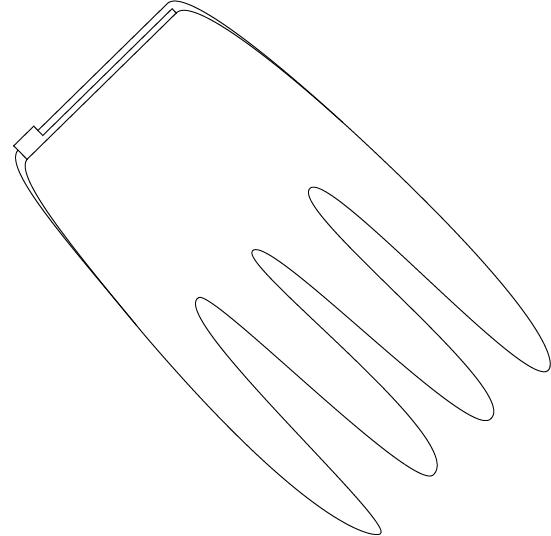
\includegraphics[scale=0.30]{images/logo_v01.png}
\end{center}

The second draft was an enhanced version of the first one. It was tried to keep it more even and linear, furthermore colors were added for the first time. This version of the logo consists of two parts, the file symbol on the top, symbolizing the body of the octopus, and four tentacles below it.

The image below shows the second sketch:

\begin{center}

\includegraphics[scale=0.30]{images/logo_v02.png}
\end{center}

This sketch became even more abstract then the first one and we got some negative feedback. Later it was replaced by an improved version, our actual logo.

\subsubsection{Current logo}

For the final version of the logo, the first concept was adopted and the idea of a folder symbol in our logo was dropped. It was decided to just include the octopus into the logo. This octopus has four visible tentacles on the front and four more in the background. At the end of these arms tags are attached.

The outcome can be seen below:


\begin{center}
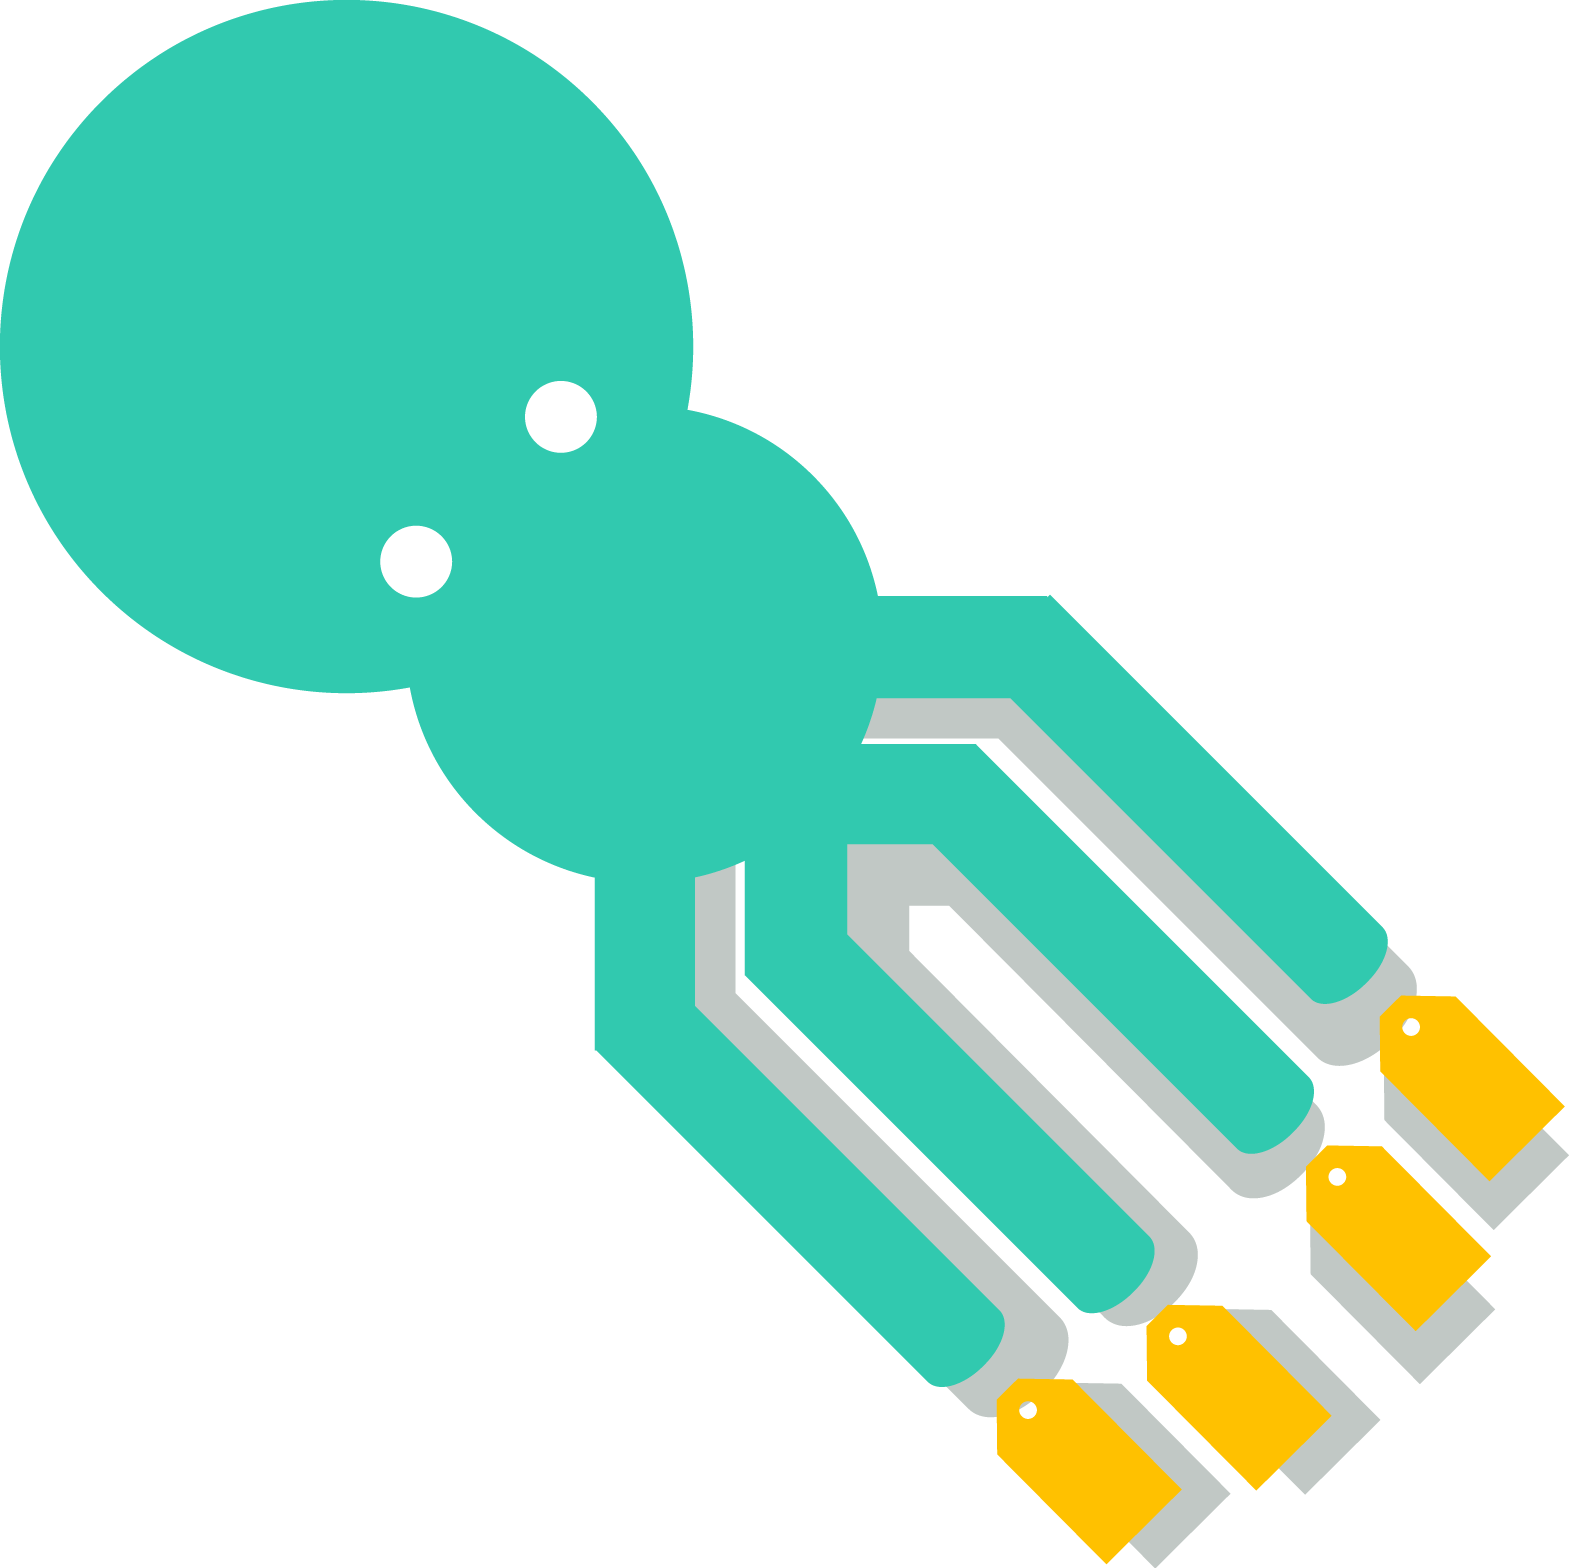
\includegraphics[width=0.5\linewidth]{images/logo.png}

A version including the project name is also available:

\includegraphics[width=\linewidth]{images/logo_text.png}
\end{center}
% TODO message -> colors
\section{Website}
%\subsection{Why is a website important?}

A website is the most efficient way to represent the product as well as the project team. In case of OctoTagger the website also fulfils the task to distribute the product by offering a download. As web developer it's necessary to keep the target audience in mind and adjust the website to its needs.

\subsection{Concept of OctoTagger website}

The website of OctoTagger follows simple and decent design guidelines. It was designed to satisfy the users needs and being as lightweight as possible at the same time. Only few and small images are used on the entire site keeping loading times short.

A major aspect of the website is the ultra-lightweight, straight and modern design. The image design was kept clear and simple without the use of explicit borders. Due to that images appear flat and homogeneous.

\subsubsection{Usability}

The site was developed to be intuitive and easy to use. The user can reach every page independent of his current position.

To make navigation easier, clickable items were made as distinctive as possible. Only buttons and elements of the navigation bar respond to mouse clicks. These objects are also the only ones to respond to hovering, so the user gets signalled that after a click an action will be performed.

As an example for usability, downloading Octotagger could hardly be easier. Every button leading to a download, is colored in a shade of green, compared to other buttons colored in a shade of blue. In fact the user just has to click every green button, follow some installation instructions and is able to use Octotagger after a few minutes.

\subsubsection{Responsive Design}

The challenge for web development is to create a website, that looks good on every available screen size and device like desktop PCs, tablets, phablets and mobile phones. This can be ensured through different solutions.

The first option is to write different CSS sheets for every screen size or device, which requires the most work.

An easier possibility is called responsive design and there are numerous frameworks to support the developer with it. 

Responsive design means that a website is created to work on every device and adapts its appearance based on the screen size and orientation. The concept is based on flexible grids and layouts and the use of CSS media queries.

The following images show the OctoTagger website adapted to different screen sizes:

\begin{center}
\begin{tabular}{ c  c c }
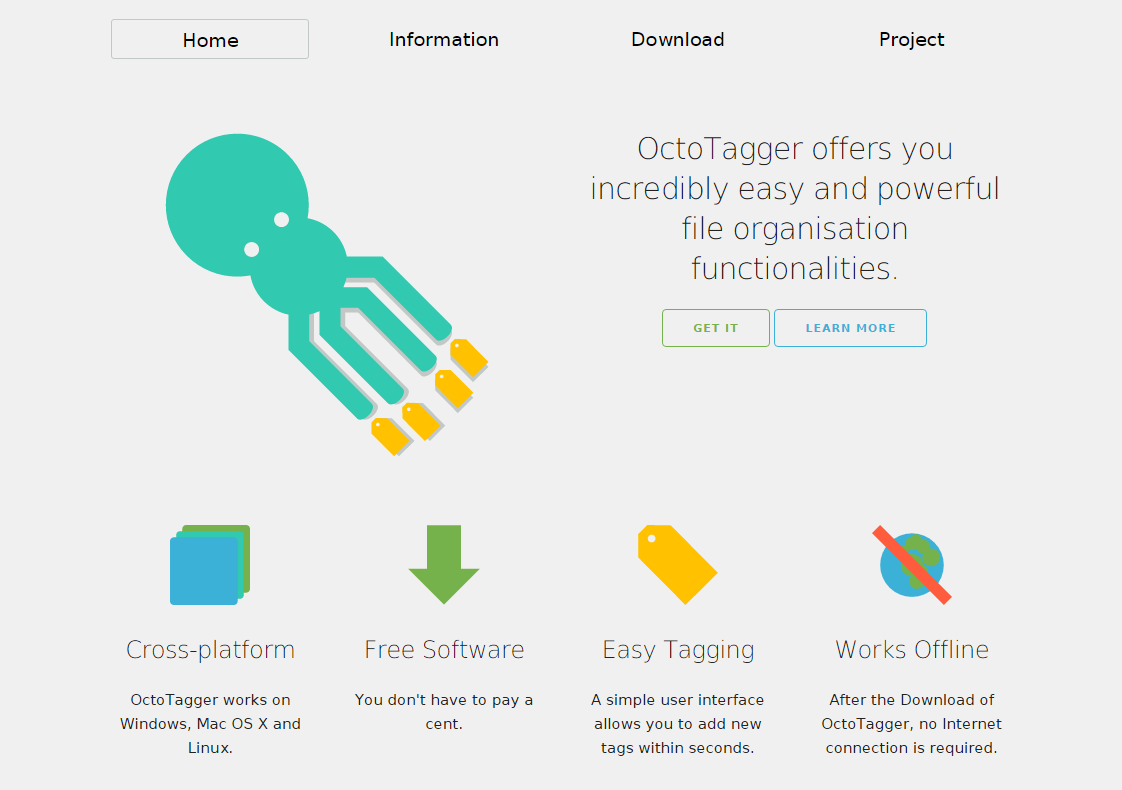
\includegraphics[scale=0.20]{images/home_full.png} & 
\includegraphics[scale=0.30]{images/resize.png} & 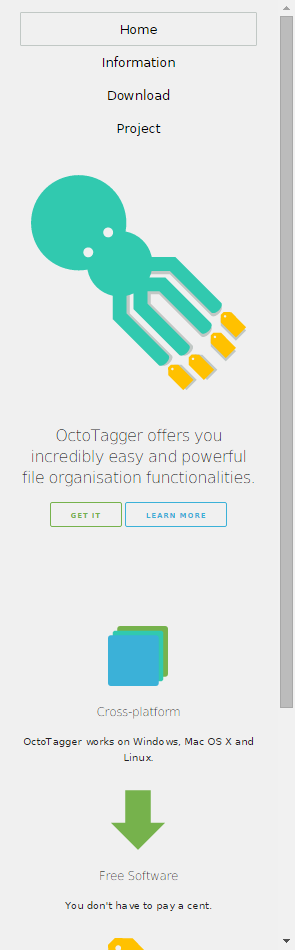
\includegraphics[scale=0.30]{images/home_small.png} \\
\end{tabular}
\end{center}

When the website passes a threshold during the resize, the elements are positioned above each other to fit the smaller screen width. The framework (see \ref{sec:Skeleton}) stacked the elements automatically, but adjustments were still necessary. Some media queries (see \ref{sec:MediaQueries}) had to be adapted so that elements fit perfectly together.

\paragraph{Flexible Grid} \hspace{0pt} \\

Most responsive framework rely on a flexible grid system, with typically 12 columns. Elements in the HTML code can now be positioned within this grid with the help of CSS classes. Depending on the width you want a HTML object to have, you have to give the proper CSS classes.

The image below shows a flexible grid example using the Skeleton framework (see \ref{sec:Skeleton})

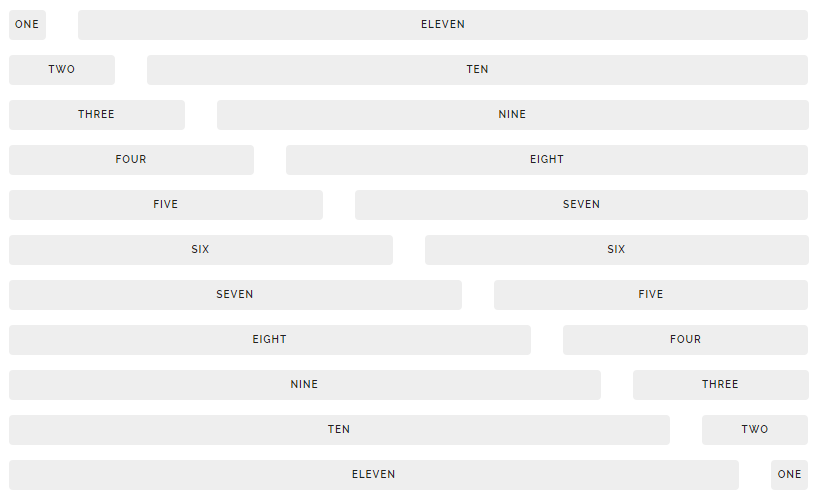
\includegraphics[scale=0.50]{images/skeleton_grid.png} 

\paragraph{CSS Media Queries} \hspace{0pt} \\
\label{sec:MediaQueries}

With the help of CSS Media Queries it's possible to set CSS attributes depending on conditions like screen width and device type. For instance the width of a box can  be increased when the window is enlarged.

The following code snippet shows an example for some width dependant media queries.

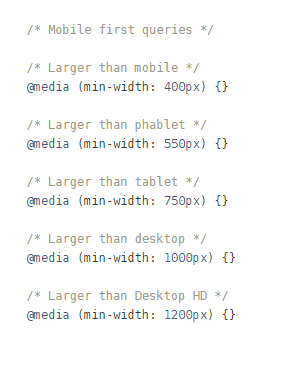
\includegraphics[scale=0.70]{images/media_query.png} 

\subsection{Structure}

The OctoTagger website is basically made up of four pages called Home, Information, Download and Project. All these pages are accessible via the navigation bar which is positioned on the top on every page. In addition there are several sub-pages only accessible on the download site.

\subsubsection{Home page}

\begin{center}
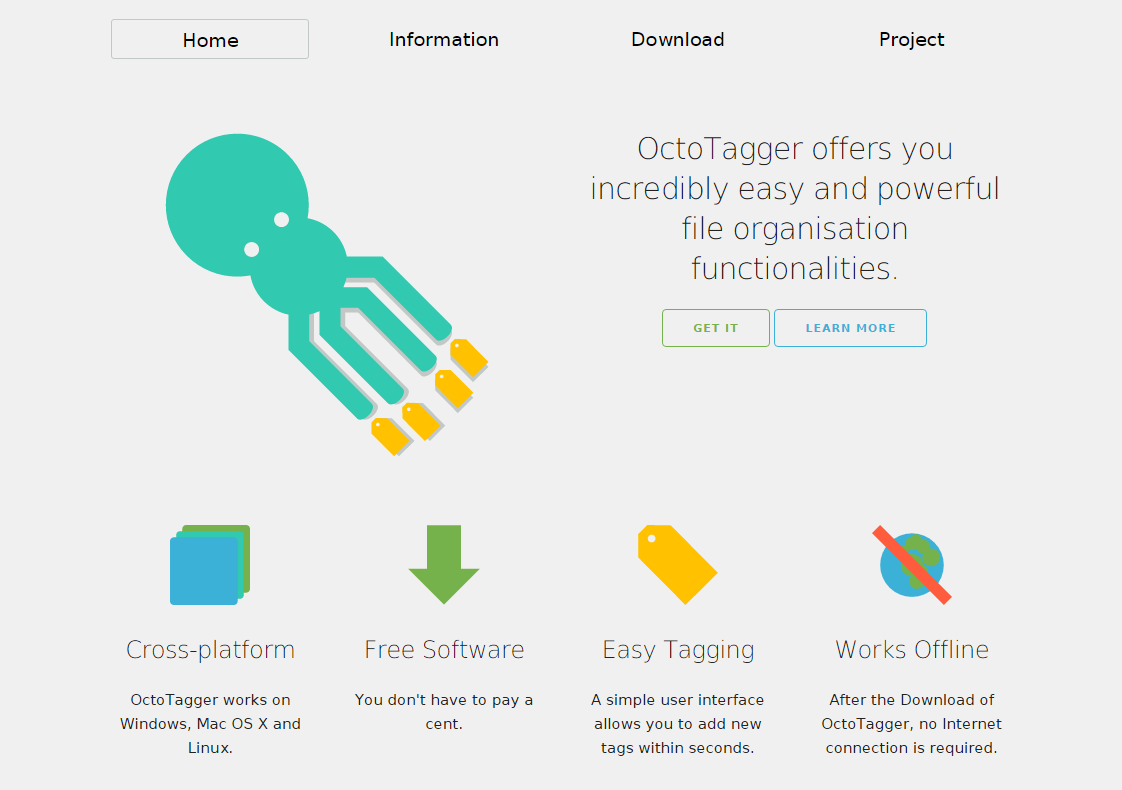
\includegraphics[scale=0.35]{images/home_full.png}\\
\end{center}

The home page is the first thing a user sees when he visits octotagger.co. This page is designed to catch the users attention with the help of a catchy slogan. The button "Learn more" is linked to the information page and with the help of the button "Get it" the user gets transferred to the download page. By just hovering the "Get it" button, a drop down menu appears and offers the possibility to directly download OctoTagger for the users operating system (see \ref{sec:OSdetection}). This option just makes sense, when the user has already installed the required software, of course.

In the bottom part the highlights of the software are pointed out with pictograms and short descriptions. The goal is to show the user the advantages of the software in one glance.

\subsubsection{Information page}

\begin{center}
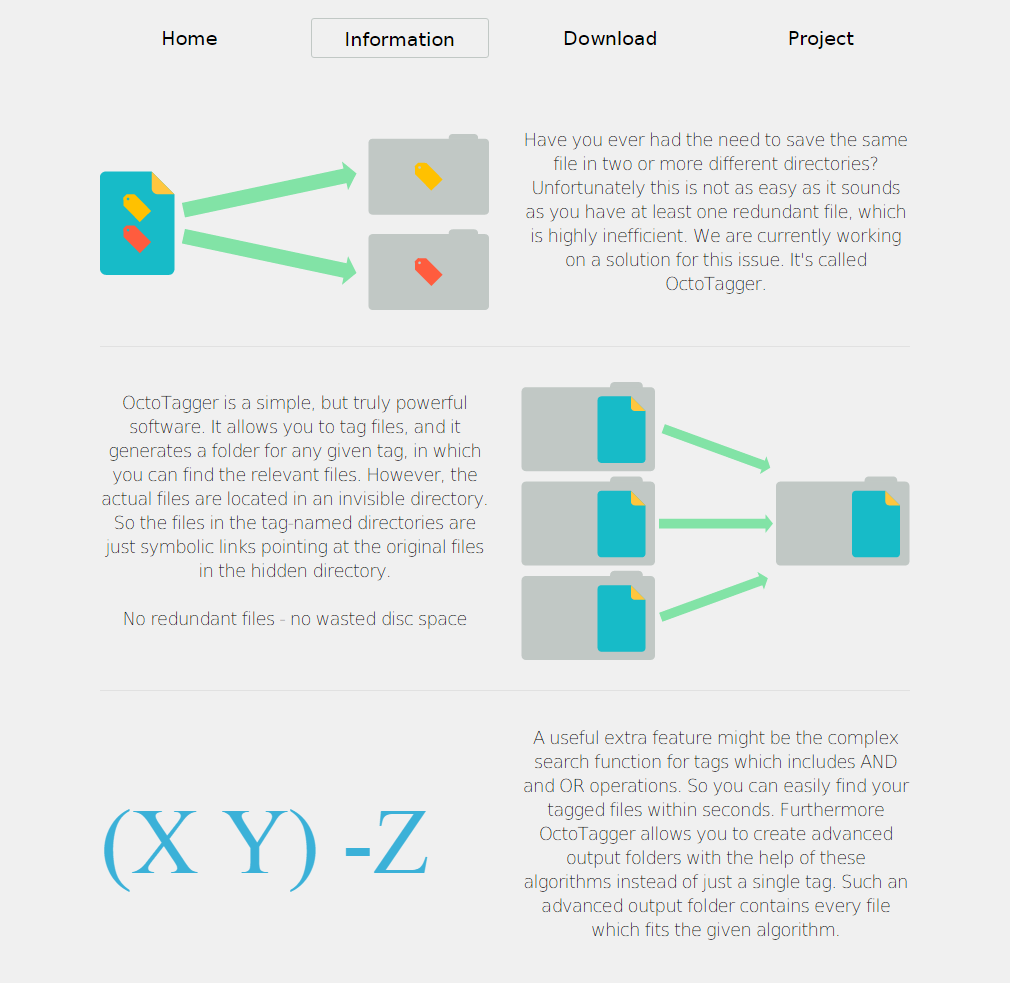
\includegraphics[scale=0.35]{images/information_full.png}
\end{center}

The information page offers the user some basic information about the functionality of OctoTagger. For this purpose, some simple images with short explanation text is shown. There is no previous knowledge needed to understand the explanation and the user doesn't have to deal with technical details.

\subsubsection{Download page}

\begin{center}
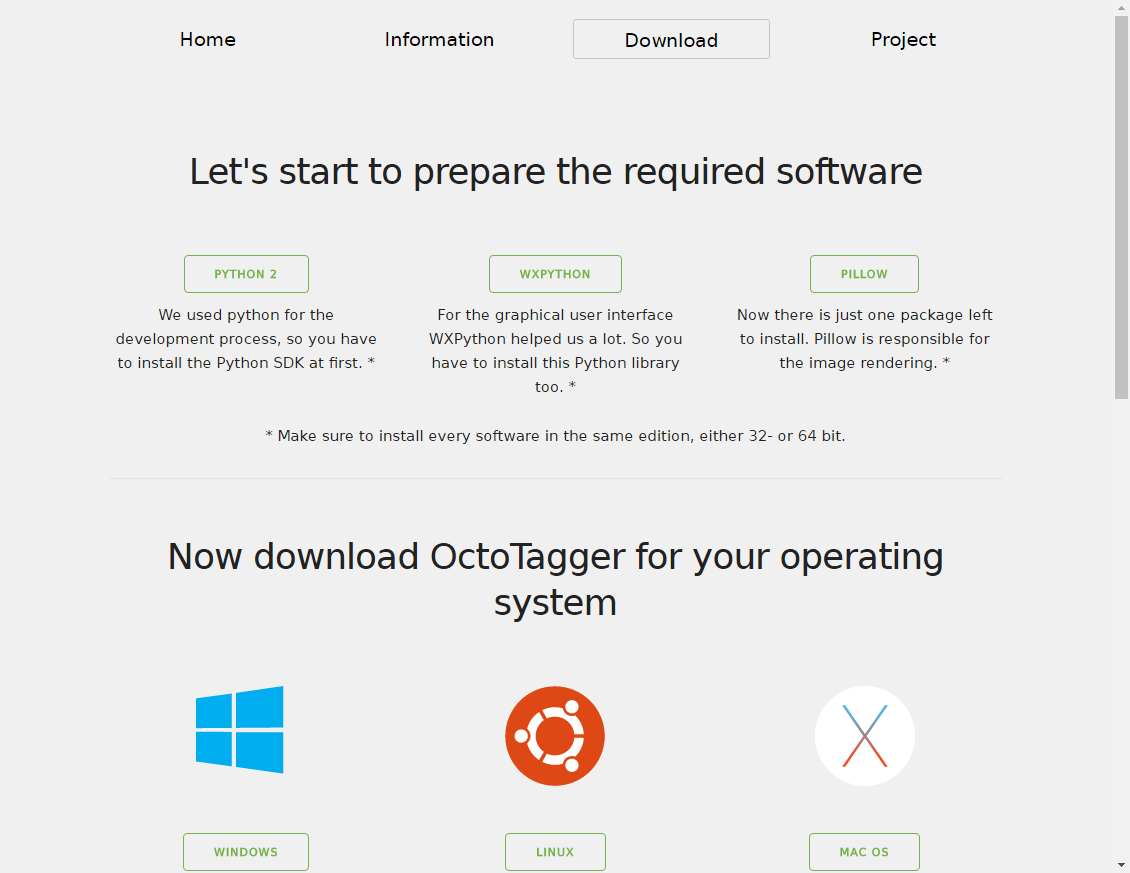
\includegraphics[scale=0.35]{images/download_full.png}
\end{center}

This page contains every available download and instructions for the installation. It's built like a step by step tutorial to guide the user through the entire process.

At first the user has to install the required software. The buttons on the top link to the developer website of the software. When a button is hovered, a dropdown menu shows up and offers further information. When the button is clicked the download site opens in a new tab.
 
The second step describes the installation of OctoTagger itself. These download buttons also provide hover functionality, which offers links to the installation guide. By clicking the download button the download starts directly. Windows user also have to install additional software to be able to use OctoTagger, which is described in the installation guide. 

In addition the user also has the possibility to download only Pywinlink, which is a service allowing symbolic links without the need of administrator rights. This service is required for OctoTagger on Windows, but is already included into the download above.

In the last step the user can download the user manual as PDF.

On the bottom of the page a link to the project Git repository can also be found.

\subsubsection{Project page}

\begin{center}
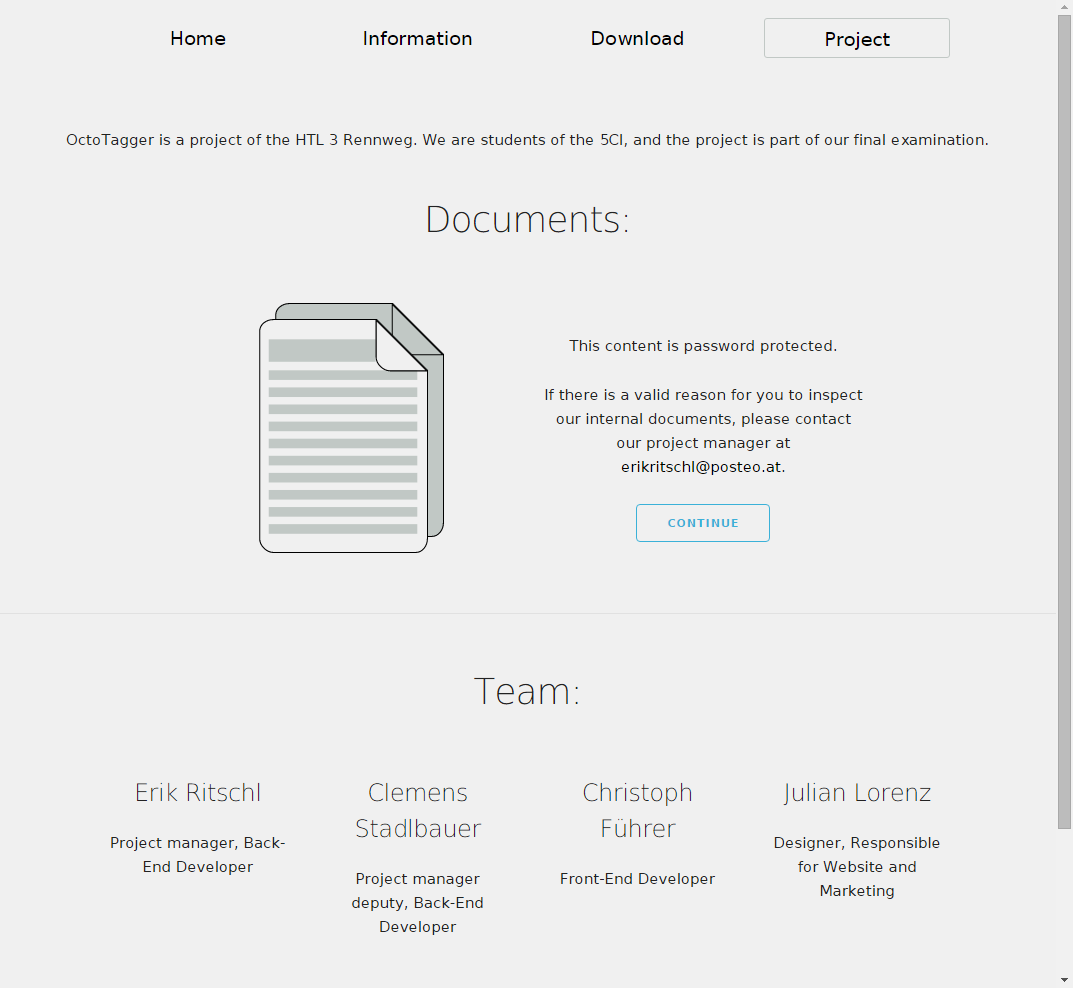
\includegraphics[scale=0.35]{images/project_full.png}
\end{center}

On this page information about the team, contact details and a link to some of our internal documents are brought together. 

\subsection{Used Tools and Technologies}

The following software, tools and frameworks helped us a lot at developing the website. Large and complex frameworks have completely been avoided to reduce loading times.


\subsubsection{Skeleton (Responsive CSS Framework)}
\label{sec:Skeleton}

Skeleton (http://getskeleton.com) is a framework which supports you with responsive development. Its source code consists of extremely few lines of code, making it great for small websites. Because of that Skeleton requires a lot of work of the developer and is basically only capable of managing the responsive grid system. It's everything you would need for responsive design, but nothing more.

\subsubsection{Adobe Illustrator}

This vector graphics editor was used for the creation of the images. 

\subsubsection{Sublime Text (Editor)}

\subsubsection{Operation System detection}
\label{sec:OSdetection}

Javascript allows the developer to check the user's operating system within just one line of code.



\subsection{Hosting}

The server is operated by the cloud provider Cloudatcost. This provider was chosen due to positive experiences in past projects and the possibility to buy a server for all time by a one-time payment. In addition, the price of 35 \$ for a simple web server is affordable for our project team. 

The server provides more then enough processing power for our needs and it's possible to install every available software on it thanks to command line control.

Namecheap was our choice concerning the purchase of the domain. This made another 8.88 \$ to use octotagger.co for one year.
% TODO like module

\section{Qualitymanagement}
\def \kapitelautor {Julian Lorenz}
% TODO


\chapter{Challenges}
\def\kapitelautor{Clemens Stadlbauer}
\label{ch:mod:challanges}
\section{wxWidgets}

Early during development the team struggled with wxWidgets. It seemed far to
difficult and time consuming creating even the simplest widgets. This was
caused by the sparse understanding of wxWidgets' methodology the team had at
that point in time.

But this misunderstanding was not to last, as every member of the team is a
quick learner; realizing that wxWidgets provides building blocks instead of
finished widgets took only a few days. Growing comfortable with the API and
learning the tricks of wxWidgets both helped with not only solving this problem
but also with speeding up development.

\section{Windows}

OctoTagger was planned to be cross-platform from the start, but the team
already knew that symlinks are not as easy on Windows as they are on other
platforms. This is the reason why one team member --- Christoph Führer --- was
assigned with the special task of finding a solution to creating symlinks on
Windows.

Throughout the development solutions kept being discovered at a steady pace.
Each one of them has been analysed, understood and tested with the product,
but, unfortunately, none of the solutions worked. The general problem seems to
be that all the answers and solutions discovered are outdated and no longer
apply.

The only option left was to create a new and working solution to this problem.
Hints, technologies and various code snippets kept coming up during the
research, though never as concrete as the other solutions, and were finally
used to implement \emph{pywinlink}. For more details on how it was implemented
see \cref{subsec:mod:pywinlink}.

\section{Mac OS X}

It was assumed from the start that there would be no large differences between
Ubuntu and Mac OS X regarding implementation. Which was true for the most part.
However, there were still some challenges. One of the biggest issues was
that there had been problems with installing \emph{wxPython}  under the newest 
version of OS X, because Apple apparently changed the structure of installer packages,
and the installer offered by \url{http://wxpython.org/} is out of date. The only solution to this problem was to manually repackage the source files in a way that allowed the software to be installed, by following the instructions on this blog entry: \url{http://davixx.fr/blog/2016/01/25/wxpython-on-os-x-el-capitan/}.

Aside from some minor GUI and behaviour differences for which the code had to be adjusted slightly, there was also the issue of creating a shortcut, which is described in more detail in \cref{sub:mod:install}. But the biggest hurdle was definitely testing, since none of our team members own an Apple PC. Computers had to be borrowed from friends and family, and where not available all the time. That is why bugs on OS X were always discovered relatively late. But all in all, we were right with our assumption that the differences between Linux and OS X aren't that large, and there were a lot less problems than with Windows.

\chapter{Evaluation}
\def\kapitelautor{Julian Lorenz}
\section{Goals}

\section{Lessons Learned}
\def\kapitelautor{}

\subsection{Erik Ritschl}
\subsection{Clemens Stadlbauer}

I have learned quite a lot about the pitfalls a project can have while working
on OctoTagger. The most important aspect, to me at least, is the continuous
ensurance of quality. Defining a small set of absolutely mandatory goals at the
beginning that capture the vision of the project, creating a functional
prototype that tests all requirements and writing automated tests to prevent
regressions from happening.

Having a clear vision from the start discourages implementing features which do
not align with this vision. We did not have such a fixed vision and I noticed
from time to time newly implemented features that seemed a bit out of place
because everyone had their own idea of what the software should do. The source
code as well should be structured so that it represents the vision resulting
in a module tree that represents how the product functions. For OctoTagger we
did not define a module layout and now we have just a bunch of files that are
difficult to manage.

Each external technology a program uses can break in unexpected ways. For this
reason a prototype is crafted, to see if all technologies really do solve our
problems instead of introducing new ones. I always though a prototype only has
to test functionality but there is one more aspect it must have: it must fulfill
all the requirements of the project. For OctoTagger a prototype showing that
managing tagged files is possible was created but some assumptions, mainly about
symlinks on Windows, were made that have not been clearly defined in the
contract. Had we not made assumptions here we would have saved a lot of time.

During development bugs appeared, which we anticipated, but as we neared
project completion fixing bugs became more difficult due to everything being
fragile. Fixing one bug resulted in breaking multiple other, previously working
parts of the software. Most of these regression bugs were in the frontend
because none of us are experts in wxWidgets but it nonetheless showed me the
importance of pinning down correct behavior with a test.

\subsection{Christoph Führer}
\subsection{Julian Lorenz}

\section{Summary}


\chapter{The Future\ldots}
\section{...of OctoTagger}

OctoTagger, the school project, ends here. But OctoTagger, the file organization software, goes on. 

We know that there is still room for many improvements in performance and usability. We also have a long list of planned features, that will greatly enhance the user experience.
The first step will be to get as many people as possible to try out OctoTagger, and collect feedback from them. Based on that, we will implement new features and change or optimize existing ones. 

We also want to try and find new use cases (e.g. archiving) and target a broader audience, which will hopefully lead to greater popularity and adaption of OctoTagger.

\section{...of pywinlink}

Pywinlink is a side product of OctoTagger, and was created out of necessity and frustration with Window's handling of symbolic links. It makes sense to continue it as a separate project. We want that future projects by other developers don't get stuck at the same problem we did, and that is why the module is published on \textit{GitHub} in a separate repository, free for everyone to adapt and modify.

Pywinlink's potential is great, since we know that there is a great demand for a solution to the problem it fixes. Therefore we plan on improving the module, making it more stable and powerful, and possibly releasing versions of it in languages other than Python.

\section{...of Us}

While it is not yet clear how many of the team members want to continue with the project, at least the project leader plans to do so.

In the long run, we see OctoTagger as a hobby side project, that we will continue to improve until there is no longer a need for it. It will always be a great thing to have in our \textit{curricula vitae}. Should the interest in OctoTagger be great enough, we could also consider to accept donations. Other forms of monetization are very unlikely, since OctoTagger is, and always will be, completely free software.

\clearpage
\def\kapitelautor{}
\appendix

\chapter{Appendix}

\printindex{}

\bibliographystyle{plaindin}
\bibliography{thesis}

\begin{thebibliography}{999}
	\bibitem{osacompile} \tfcode{osacompile} man page:
	
	\url{https://developer.apple.com/library/mac/documentation/Darwin/Reference/ManPages/man1/osacompile.1.html}
	
	\bibitem{AppleScript} AppleScript: 
	
	\url{https://developer.apple.com/library/mac/documentation/AppleScript/Conceptual/AppleScriptX/AppleScriptX.html}
	\bibitem{EnvironmentVariables} Explanation of environment variables:  
	
	\url{https://en.wikibooks.org/wiki/Guide_to_Unix/Environment_Variables}
\end{thebibliography}

\end{document}
